\documentclass[tikz,border=4pt]{standalone}
\usepackage{amsmath}
\begin{document}
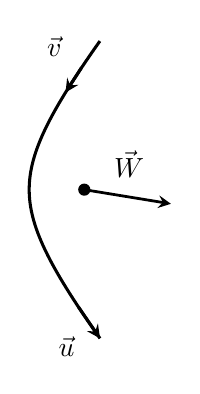
\begin{tikzpicture}[>=stealth, thick, scale=1.0]
  % Hyperbolic probe trajectory curving around planet
  \draw[line width=1.1pt, domain=-1.35:1.35, samples=80]
    plot ({-1.2 + 0.85*cosh(\x)}, {1.05*sinh(\x)});

  % Incoming velocity arrow v (upper right, heading down-left)
  \draw[->, line width=1.1pt]
    ({-1.2 + 0.85*cosh(1.18)}, {1.05*sinh(1.18)}) -- ({-1.2 + 0.85*cosh(1.00)}, {1.05*sinh(1.00)});
  \node[above left] at ({-1.2 + 0.85*cosh(1.12) - 0.05}, {1.05*sinh(1.12) + 0.12}) {$\vec{v}$};

  % Outgoing velocity arrow u (lower right, heading down-right)
  \draw[->, line width=1.1pt]
    ({-1.2 + 0.85*cosh(-1.15)}, {1.05*sinh(-1.15)}) -- ({-1.2 + 0.85*cosh(-1.35)}, {1.05*sinh(-1.35)});
  \node[below left] at ({-1.2 + 0.85*cosh(-1.25) - 0.05}, {1.05*sinh(-1.25) - 0.05}) {$\vec{u}$};

  % Planet dot and velocity vector W
  \fill (0.35, 0) circle (2.2pt);
  \draw[->, line width=1.0pt] (0.35, 0) -- (1.45, -0.18);
  \node[above] at (0.92, 0.02) {$\vec{W}$};
\end{tikzpicture}
\end{document}
